%=================================================================
% CSE 4345 — Big Data Analytics
% Week 9, Part 1: Data Visualization —
%                 Principles, Techniques, and Big Data Visualization Tools
% Department of CSE, Premier University
%
% Part 1 covers: Tufte's principles (data-ink ratio, small multiples)
%               · Shneiderman's mantra and taxonomy · Chart selection by data type
%               · Overplotting · Pre-aggregation and data cubes
%               · Streaming visualization · Tools landscape
%               · Ivy League alignment · Assessment
% Part 2 covers: Tufte (1983), Shneiderman (1996), Bostock et al. (2011)
%               · NYT Graphics Desk case study
%=================================================================

\documentclass[aspectratio=169,10pt]{beamer}

%---------- Packages ----------
\usepackage[utf8]{inputenc}
\usepackage[T1]{fontenc}
\usepackage{booktabs}
\usepackage{xcolor}
\usepackage{tikz}
\usetikzlibrary{shapes.geometric, positioning, arrows.meta,
                decorations.pathreplacing, calc, fit, backgrounds,
                patterns}
\usepackage{amsmath}
\usepackage{graphicx}
\usepackage{multicol}
\usepackage{enumerate}
\usepackage{array}
\usepackage{listings}

%---------- Theme ----------
\usetheme{Madrid}

%---------- Premier University Color Identity ----------
\definecolor{PUNavy}{RGB}{10,36,99}
\definecolor{PUGold}{RGB}{197,151,37}
\definecolor{PULightBlue}{RGB}{210,228,255}
\definecolor{PUTeal}{RGB}{0,100,100}
\definecolor{PUGray}{RGB}{90,90,90}
\definecolor{PURed}{RGB}{160,30,30}
\definecolor{PUGreen}{RGB}{30,120,60}
\definecolor{PUOrange}{RGB}{200,100,20}
\definecolor{PUPurple}{RGB}{80,0,120}

\setbeamercolor{palette primary}{bg=PUNavy, fg=white}
\setbeamercolor{palette secondary}{bg=PUNavy!85, fg=white}
\setbeamercolor{palette tertiary}{bg=PUNavy!70, fg=white}
\setbeamercolor{palette quaternary}{bg=PUNavy, fg=white}
\setbeamercolor{structure}{fg=PUNavy}
\setbeamercolor{title}{bg=PUNavy, fg=PUGold}
\setbeamercolor{subtitle}{fg=white}
\setbeamercolor{frametitle}{bg=PUNavy, fg=PUGold}
\setbeamercolor{alerted text}{fg=PUGold!85!black}
\setbeamercolor{block title}{bg=PUNavy, fg=white}
\setbeamercolor{block body}{bg=PULightBlue!45}
\setbeamercolor{block title alerted}{bg=PUGold!80!black, fg=white}
\setbeamercolor{block body alerted}{bg=PUGold!12}
\setbeamercolor{block title example}{bg=PUTeal, fg=white}
\setbeamercolor{block body example}{bg=PUTeal!10}
\setbeamercolor{section in toc}{fg=PUNavy}
\setbeamercolor{itemize item}{fg=PUGold!80!black}
\setbeamercolor{itemize subitem}{fg=PUNavy!70}

\setbeamertemplate{navigation symbols}{}
\setbeamertemplate{itemize item}{\scriptsize\raise1.5pt\hbox{\textbullet}}
\setbeamertemplate{itemize subitem}{\scriptsize\raise1pt\hbox{--}}

%---------- Code listing style ----------
\lstset{
  basicstyle=\ttfamily\scriptsize,
  backgroundcolor=\color{PUNavy!8},
  frame=single, rulecolor=\color{PUNavy!30},
  breaklines=true, language={},
  keywordstyle=\color{PUNavy}\bfseries,
  commentstyle=\color{PUGray}\itshape,
  stringstyle=\color{PUGreen!70!black},
}

%---------- Section separator ----------
\AtBeginSection[]{
  \begin{frame}[plain]
    \vfill\centering
    \begin{beamercolorbox}[sep=12pt,center,shadow=true,rounded=true]{block title}
      \usebeamerfont{title}\insertsectionhead\par
    \end{beamercolorbox}
    \vfill
  \end{frame}
}

%---------- Title metadata ----------
\title[CSE 4345 \textbar{} Week 9, Part 1]{CSE 4345: Big Data Analytics}
\subtitle{Week 9, Part 1 \textemdash\ Data Visualization:
  Principles, Techniques \& Big Data Tools}
\author[Dept.\ of CSE]{Department of Computer Science \& Engineering\\[4pt]
       \small Premier University, Chittagong}
\institute{}
\date{Semester 2026}

%=================================================================
\begin{document}
%=================================================================

\begin{frame}\titlepage\end{frame}

%----------------------------------------------------------------
\begin{frame}{Course \& Lecture Information}
  \begin{columns}[T]
    \column{0.47\textwidth}
      \begin{block}{Lecture Identity}
        \begin{tabular}{ll}
          \textbf{Course:}      & CSE 4345 \\
          \textbf{Week / Part:} & 9 of 11 \textbar\ Part 1 of 2 \\
          \textbf{CLO:}         & CLO3 \\
          \textbf{PLO:}         & PLO(e) \\
        \end{tabular}
      \end{block}
      \vspace{6pt}
      \begin{alertblock}{CLO3}
        \textit{``Explain the importance and performance of different big data techniques and tools used to store, manage, and analyse large datasets''}
      \end{alertblock}
      \vspace{6pt}
      \begin{block}{Course Progression}
        \small
        Week 7: Hive, HiveQL, SQL-on-Hadoop\\
        Week 8: Kafka, Sqoop, Flume, Lambda/Kappa\\
        \textbf{Week 9: Visualization principles and tools}\\
        Week 10: Social media, time series, health data
      \end{block}

    \column{0.50\textwidth}
      \begin{exampleblock}{Part 1 Covers}
        \begin{itemize}
          \item Why visualization is a critical skill in big data analytics
          \item Tufte's principles: data-ink ratio, small multiples, sparklines
          \item Shneiderman's visualization mantra and seven task taxonomy
          \item Choosing the right chart by data type
          \item Big data visualization challenge 1: overplotting (hexbin, density contour)
          \item Big data visualization challenge 2: latency (pre-aggregation, data cubes)
          \item Big data visualization challenge 3: streaming (real-time chart updates)
          \item Tools landscape: Tableau, Power BI, D3.js, Grafana, Superset, Kibana
          \item Streaming visualization architecture (Kafka $\to$ WebSocket $\to$ browser)
          \item Ivy League alignment
          \item Student assessment pool
        \end{itemize}
      \end{exampleblock}
  \end{columns}
\end{frame}

\begin{frame}{Lecture Agenda}\tableofcontents\end{frame}

%================================================================
\section{Why Visualization Matters in Big Data}
%================================================================

\begin{frame}{From Data to Insight: The Visualization Imperative}
  \begin{columns}[T]
    \column{0.52\textwidth}
      \begin{block}{Anscombe's Quartet (1973)}
        Four datasets with \textbf{identical summary statistics} (mean, variance, correlation $r = 0.816$) that look completely different when plotted.  This 50-year-old demonstration remains the canonical argument for always visualising data before trusting statistics.
        \vspace{4pt}
        \begin{center}
        \renewcommand{\arraystretch}{1.2}
        \begin{tabular}{lcc}
          \toprule
          & \textbf{All 4 datasets} \\
          \midrule
          Mean of $x$ & 9.0 \\
          Mean of $y$ & 7.5 \\
          Variance of $x$ & 11.0 \\
          Correlation $r$ & 0.816 \\
          Linear fit & $y = 3 + 0.5x$ \\
          \bottomrule
        \end{tabular}
        \end{center}
        Yet Dataset I is linear, II is curved, III has an outlier, and IV is a vertical cluster --- \textbf{identical numbers, four different stories}.
      \end{block}

    \column{0.45\textwidth}
      \begin{alertblock}{The Big Data Dimension}
        \small At petabyte scale, summary statistics are even more dangerous because:
        \begin{itemize}
          \item A single table with 10 billion rows may contain multiple overlapping populations with opposite trends that average out
          \item Log-scale distributions (income, city size, web traffic) make arithmetic means meaningless
          \item Streaming data can hide sudden regime changes that a daily average obscures
        \end{itemize}
        \textbf{Visualization is the first and most powerful quality check on any big data analysis.}
      \end{alertblock}
      \vspace{6pt}
      \begin{exampleblock}{Bangladesh Example}
        \small DGHS monthly disease count averages look stable year-over-year.  A time-series line chart immediately reveals a \textbf{seasonal cholera spike} every June--August (monsoon) and a \textbf{dengue peak} every October --- patterns invisible in the annual mean.
      \end{exampleblock}
  \end{columns}
\end{frame}

%================================================================
\section{Tufte's Principles of Analytical Design}
%================================================================

\begin{frame}{Tufte: Maximise the Data-Ink Ratio}
  \begin{columns}[T]
    \column{0.50\textwidth}
      \begin{block}{The Three Core Principles (Tufte, 1983)}
        \begin{enumerate}
          \item \textbf{Data-ink ratio:}  Of all the ink used in a chart, maximise the fraction that encodes actual data.  Eliminate ``chart junk'' --- decorative borders, 3D effects, gradient fills, redundant legends, unnecessary gridlines.
          \vspace{4pt}
          \[\text{Data-ink ratio} = \frac{\text{ink encoding data}}{\text{total ink in chart}}\]
          \vspace{2pt}
          \item \textbf{Small multiples:}  Repeat the \textit{same} chart structure across different subsets (districts, years, categories) for direct visual comparison.  The eye detects differences and trends across a grid of small charts far more quickly than by reading separate tables.
          \item \textbf{Sparklines:}  Word-sized data graphics embedded in text or table cells.  A sparkline next to a number adds temporal context without requiring a separate figure.
        \end{enumerate}
      \end{block}

    \column{0.47\textwidth}
      \begin{center}
      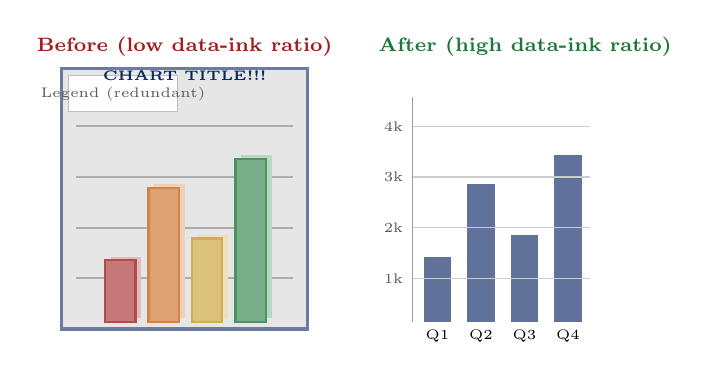
\begin{tikzpicture}[scale=0.92]
        % ---- Before: chart junk ----
        \node[font=\scriptsize\bfseries, PURed] at (-1.5, 4.7) {Before (low data-ink ratio)};
        % 3D-ish background
        \fill[PUGray!15] (-3.2, 0.8) rectangle (0.2, 4.4);
        % Thick grid lines
        \foreach \y in {1.5, 2.2, 2.9, 3.6} {
          \draw[PUGray!50, thick] (-3.0,\y)--(0.0,\y);
        }
        % 3D bars (shadow + bar)
        \foreach \x/\h/\c in {-2.6/1.8/PURed, -2.0/2.8/PUOrange,
                               -1.4/2.1/PUGold, -0.8/3.2/PUGreen} {
          \fill[\c!30] (\x+0.08, 0.95) rectangle (\x+0.5, \h);
          \fill[\c!60] (\x, 0.9) rectangle (\x+0.42, \h-0.05);
          \draw[\c!80, thick] (\x, 0.9) rectangle (\x+0.42, \h-0.05);
        }
        % Decorative border
        \draw[PUNavy!60, very thick] (-3.2, 0.8) rectangle (0.2, 4.4);
        % Legend box
        \fill[white] (-3.1, 3.8) rectangle (-1.6, 4.3);
        \draw[PUGray!40] (-3.1, 3.8) rectangle (-1.6, 4.3);
        \node[font=\tiny, PUGray] at (-2.35, 4.05) {Legend (redundant)};
        % Title clutter
        \node[font=\tiny\bfseries, PUNavy] at (-1.5, 4.3) {CHART TITLE!!!};

        % ---- After: clean ----
        \node[font=\scriptsize\bfseries, PUGreen] at (3.2, 4.7)
              {After (high data-ink ratio)};
        \foreach \x/\h in {1.8/1.8, 2.4/2.8, 3.0/2.1, 3.6/3.2} {
          \fill[PUNavy!65] (\x, 0.9) rectangle (\x+0.38, \h);
        }
        % Minimal y-axis
        \draw[PUGray!60] (1.65, 0.9)--(1.65, 4.0);
        \foreach \y/\lbl in {1.5/1k, 2.2/2k, 2.9/3k, 3.6/4k} {
          \draw[PUGray!30] (1.65,\y)--(4.1,\y);
          \node[font=\tiny, PUGray, left] at (1.65,\y) {\lbl};
        }
        % x-labels only
        \foreach \x/\lbl in {1.99/Q1, 2.59/Q2, 3.19/Q3, 3.79/Q4} {
          \node[font=\tiny] at (\x, 0.7) {\lbl};
        }
      \end{tikzpicture}
      \end{center}
      \vspace{-2pt}
      \begin{alertblock}{Rule}
        \small If erasing an element does not reduce the information in the chart, erase it.
      \end{alertblock}
  \end{columns}
\end{frame}

%----------------------------------------------------------------
\begin{frame}{Tufte: Small Multiples and Sparklines}
  \begin{columns}[T]
    \column{0.50\textwidth}
      \begin{block}{Small Multiples}
        \small A small multiple (also called a \textbf{trellis} or \textbf{facet} chart) repeats the same visual structure across partitions of the data.  The result is a grid where the eye can instantly compare trends:
        \vspace{4pt}
        \begin{center}
        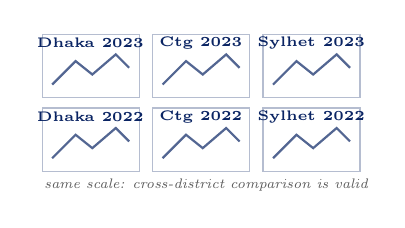
\begin{tikzpicture}[scale=0.85]
          \foreach \col/\district in {0/Dhaka, 1/Ctg, 2/Sylhet} {
            \foreach \row/\yr in {0/2022, 1/2023} {
              \pgfmathsetmacro{\bx}{(\col)*1.65}
              \pgfmathsetmacro{\by}{(\row)*1.1}
              \draw[PUNavy!30] (\bx, \by) rectangle (\bx+1.45, \by+0.95);
              \node[font=\tiny\bfseries, PUNavy] at (\bx+0.72, \by+0.82)
                    {\district\ \yr};
              % Tiny sparkline-like trend
              \draw[PUNavy!70, thick]
                    (\bx+0.15, \by+0.2)--(\bx+0.5, \by+0.55)--
                    (\bx+0.75, \by+0.35)--(\bx+1.1, \by+0.65)--
                    (\bx+1.3, \by+0.45);
            }
          }
          \node[font=\tiny\itshape, PUGray] at (2.45, -0.2)
                {same scale: cross-district comparison is valid};
        \end{tikzpicture}
        \end{center}
        \vspace{2pt}
        Each panel uses the \textbf{same axis scale} so relative magnitudes are directly comparable.
      \end{block}

    \column{0.47\textwidth}
      \begin{exampleblock}{Sparklines}
        \small Sparklines embed a trend line directly inside a table or text, eliminating the need for a separate figure.  They communicate direction and shape without requiring the reader to track a separate chart.
        \vspace{6pt}
        \begin{center}
        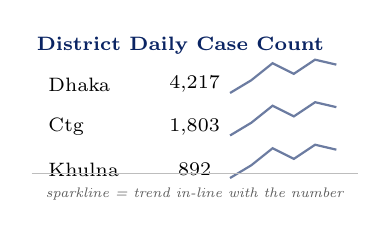
\begin{tikzpicture}[scale=0.9]
          \node[font=\scriptsize\bfseries, PUNavy] at (0, 2.2)
                {District Daily Case Count};
          \foreach \row/\dist/\val/\trendpts in {
            0/Dhaka/4{,}217/{0.3,0.5,0.8,0.6,1.0,0.9},
            1/Ctg/1{,}803/{0.8,0.6,0.5,0.3,0.4,0.2},
            2/Khulna/892/{0.2,0.3,0.2,0.4,0.3,0.5}
          } {
            \pgfmathsetmacro{\ry}{1.65 - \row*0.6}
            \node[font=\scriptsize, anchor=west] at (-2.0, \ry) {\dist};
            \node[font=\scriptsize] at (0.2, \ry) {\val};
            % Sparkline
            \draw[PUNavy!60, thick]
                  (0.7,\ry-0.12)--(1.0,\ry+0.06)--(1.3,\ry+0.3)--
                  (1.6,\ry+0.15)--(1.9,\ry+0.35)--(2.2,\ry+0.28);
          }
          \draw[PUGray!40] (-2.1,0.4)--(2.5,0.4);
          \node[font=\tiny\itshape, PUGray] at (0.2, 0.1)
                {sparkline = trend in-line with the number};
        \end{tikzpicture}
        \end{center}
      \end{exampleblock}
  \end{columns}
\end{frame}

%================================================================
\section{Shneiderman's Visualization Mantra and Taxonomy}
%================================================================

\begin{frame}{Shneiderman's Mantra and Seven Data Types}
  \begin{columns}[T]
    \column{0.50\textwidth}
      \begin{block}{The Visualization Mantra (Shneiderman, 1996)}
        \begin{center}
          \Large\textit{``Overview first,}\\
          \large\textit{zoom and filter,}\\
          \normalsize\textit{then details on demand.''}
        \end{center}
        \vspace{6pt}
        \small This three-step interaction model applies to \textbf{every} interactive visualization system.  A user should always be able to:
        \begin{enumerate}
          \item See the \textbf{whole picture} first (global context)
          \item \textbf{Narrow down} to the region or subset of interest (zoom/filter)
          \item Retrieve the \textbf{raw record} for any item when needed (drill-down)
        \end{enumerate}
        This model directly shapes modern BI tools: Tableau's drill-down, Grafana's time-range zoom, and Google Maps' zoom interaction all implement exactly this mantra.
      \end{block}

    \column{0.47\textwidth}
      \begin{exampleblock}{Shneiderman's Seven Data Types}
        {\small
        \renewcommand{\arraystretch}{1.35}
        \begin{tabular}{p{2.0cm}p{3.0cm}}
          \toprule
          \textbf{Data Type} & \textbf{Best Chart Types} \\
          \midrule
          \textbf{1D Linear}  & Bar chart, histogram \\
          \textbf{2D Map}     & Choropleth, bubble map \\
          \textbf{3D World}   & 3D scatter, volume render \\
          \textbf{Temporal}   & Line chart, area, calendar heatmap \\
          \textbf{Multi-dim}  & Scatterplot matrix, parallel coords, heatmap \\
          \textbf{Tree}       & Treemap, sunburst, dendogram \\
          \textbf{Network}    & Force-directed graph, chord diagram \\
          \bottomrule
        \end{tabular}
        }
        \vspace{4pt}
        \textbf{Five tasks} that visualizations must support:\\
        \small Overview $\cdot$ Zoom $\cdot$ Filter $\cdot$ Details-on-demand $\cdot$ Relate (cross-highlight)
      \end{exampleblock}
  \end{columns}
\end{frame}

%================================================================
\section{Choosing the Right Chart}
%================================================================

\begin{frame}{Visualization Selection by Data Type and Question}
  \centering
  \renewcommand{\arraystretch}{1.5}
  \begin{tabular}{p{2.4cm}p{3.0cm}p{5.2cm}p{1.8cm}}
    \toprule
    \textbf{Data Type} & \textbf{Analytical Question} & \textbf{Recommended Visualization} & \textbf{Avoid} \\
    \midrule
    \textbf{Temporal} &
      How did X change over time? &
      Line chart (trend), area chart (cumulative), calendar heatmap (daily pattern) &
      Pie chart \\
    \textbf{Categorical} &
      Which category is largest? &
      Horizontal bar chart ($>$5 cats); grouped bar (comparison across groups) &
      3D pie chart \\
    \textbf{Geographical} &
      How is X distributed across regions? &
      Choropleth (rate/proportion); proportional bubble map (absolute count) &
      Plain bar for spatial data \\
    \textbf{Relational} &
      How are entities connected? &
      Force-directed network graph; chord diagram (flow between groups) &
      Table \\
    \textbf{Distribution} &
      What is the spread and shape of X? &
      Histogram (shape); box plot (quartiles + outliers); violin (density + quartiles) &
      Line chart \\
    \textbf{Correlation} &
      Does X predict Y? &
      Scatterplot (two variables); scatterplot matrix (pairwise all variables) &
      Bar chart \\
    \textbf{High-dimensional} &
      Any pattern across $>$3 variables? &
      Parallel coordinates; t-SNE / UMAP scatterplot; heatmap with clustering &
      3D bar chart \\
    \bottomrule
  \end{tabular}
  \vspace{4pt}
  \begin{alertblock}{\small The Most Abused Chart}
    \small \textbf{The pie chart} should only be used when there are $\leq$4 categories and the question is ``what fraction of the whole?''  For more categories, for any comparison question, or for any time series, a bar chart or line chart is \textit{always} more readable.  Humans judge angles and arc lengths far less accurately than bar lengths.
  \end{alertblock}
\end{frame}

%================================================================
\section{Big Data Visualization Challenges}
%================================================================

\begin{frame}{Challenge 1: Overplotting at Scale}
  \begin{columns}[T]
    \column{0.52\textwidth}
      \begin{block}{The Overplotting Problem}
        A standard scatterplot renders one point per data record.  At \textbf{millions of records}, points overlap completely --- the chart becomes a solid blob of ink that conveys zero information beyond ``data exists here.''
        \vspace{4pt}
        \textbf{Three solutions in increasing sophistication:}
        \begin{enumerate}
          \item \textbf{Alpha transparency (opacity):}  Set each point to $\alpha = 0.02$.  Denser regions appear darker.  Simple but still fails at very high densities.
          \item \textbf{Hexbin aggregation:}  Divide the 2D plot area into a hexagonal grid.  Count points in each hex.  Colour each hex by count.  A scatter of 10 million points becomes a grid of $\sim$10{,}000 hex cells --- interactive and readable.
          \item \textbf{Kernel Density Estimation (KDE) / 2D density contour:}  Estimate the continuous probability density of the point cloud.  Draw contour lines or filled contours at probability levels.  Reveals shape, modes, and tails clearly.
        \end{enumerate}
      \end{block}

    \column{0.45\textwidth}
      \begin{center}
      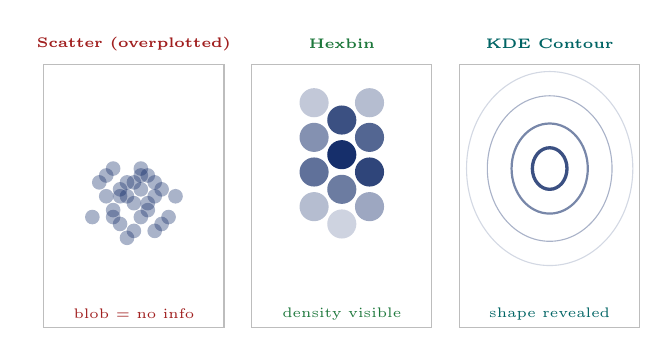
\begin{tikzpicture}[scale=0.88]
        % Panel 1: Overplotted scatter
        \node[font=\tiny\bfseries, PURed] at (-2.5, 4.5) {Scatter (overplotted)};
        \draw[PUGray!40] (-3.8,0.4) rectangle (-1.2,4.2);
        % Simulate dense blob
        \foreach \dx/\dy in {
          0/0, 0.1/0.2, -0.1/0.1, 0.2/-0.1, -0.2/0.2,
          0.3/0.1, -0.3/-0.1, 0.1/-0.2, -0.1/0.3, 0.0/0.3,
          0.4/0.2, -0.4/0.1, 0.2/0.4, -0.2/-0.3, 0.5/-0.2,
          -0.5/0.3, 0.3/-0.4, -0.3/0.5, 0.6/0.1, -0.6/-0.2,
          0.1/0.5, -0.1/-0.5, 0.4/-0.3, -0.4/0.4, 0.0/-0.4,
          0.2/0.0, -0.2/0.1, 0.3/0.3, -0.3/-0.2, 0.1/0.4
        } {
          \fill[PUNavy, opacity=0.35] (-2.5+\dx, 2.2+\dy) circle (3pt);
        }
        \node[font=\tiny, PURed] at (-2.5, 0.6) {blob = no info};

        % Panel 2: Hexbin
        \node[font=\tiny\bfseries, PUGreen] at (0.5, 4.5) {Hexbin};
        \draw[PUGray!40] (-0.8,0.4) rectangle (1.8,4.2);
        % Hexagonal cells
        \foreach \hx/\hy/\intensity in {
          0.5/3.4/80, 0.5/2.9/95, 0.5/2.4/60,
          0.9/3.15/70, 0.9/2.65/85, 0.9/2.15/40,
          0.1/3.15/50, 0.1/2.65/65, 0.1/2.15/30,
          0.5/1.9/20, 0.9/3.65/30, 0.1/3.65/25
        } {
          \pgfmathsetmacro{\fc}{100-\intensity}
          \fill[PUNavy!\intensity] (\hx, \hy) circle (0.21cm);
        }
        \node[font=\tiny, PUGreen] at (0.5, 0.6) {density visible};

        % Panel 3: KDE contour
        \node[font=\tiny\bfseries, PUTeal] at (3.5, 4.5) {KDE Contour};
        \draw[PUGray!40] (2.2,0.4) rectangle (4.8,4.2);
        % Nested ellipses for contour
        \draw[PUNavy!80, very thick] (3.5, 2.7) ellipse (0.25cm and 0.3cm);
        \draw[PUNavy!55, thick] (3.5, 2.7) ellipse (0.55cm and 0.65cm);
        \draw[PUNavy!35] (3.5, 2.7) ellipse (0.9cm and 1.05cm);
        \draw[PUNavy!18] (3.5, 2.7) ellipse (1.2cm and 1.4cm);
        \node[font=\tiny, PUTeal] at (3.5, 0.6) {shape revealed};
      \end{tikzpicture}
      \end{center}
  \end{columns}
\end{frame}

%----------------------------------------------------------------
\begin{frame}{Challenge 2: Latency and Pre-Aggregation}
  \begin{columns}[T]
    \column{0.52\textwidth}
      \begin{block}{The Interactivity Problem}
        A business analyst using Tableau expects a dashboard filter (e.g., \textit{``show Q1 2024 only''}) to respond in under \textbf{1 second}.  But the underlying table has \textbf{100 billion rows} in Hive on HDFS.  A Hive query over 100 billion rows takes minutes, not milliseconds.
        \vspace{4pt}
        \textbf{Two solutions:}
        \begin{enumerate}
          \item \textbf{Pre-aggregation with a data cube:}  Materialise aggregate tables at all combinations of dimensions (district $\times$ date $\times$ product $\times$ channel) in advance.  Queries read from the pre-computed cube (millions of rows) rather than the raw fact table (billions of rows).
          \item \textbf{Approximate query processing (AQP):}  Return a statistically correct estimate of the aggregate in milliseconds by sampling the table.  Tools: Apache Datasketches, BlinkDB.  Trade accuracy for speed --- acceptable for dashboards but not for financial reconciliation.
        \end{enumerate}
      \end{block}

    \column{0.45\textwidth}
      \begin{center}
      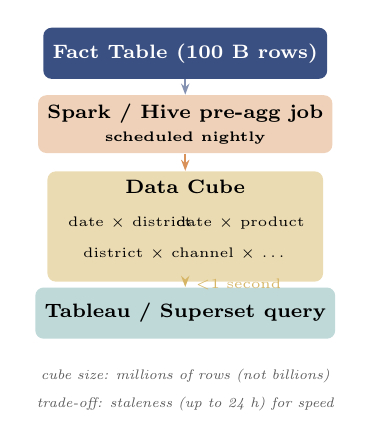
\begin{tikzpicture}[
          box/.style={rectangle, rounded corners=3pt, minimum width=3.2cm,
                      minimum height=0.65cm, font=\scriptsize\bfseries, align=center},
          arr/.style={-{Stealth[length=4pt]}, thick}
        ]
        % Raw fact table
        \node[box, fill=PUNavy!80, text=white] (raw) at (0, 4.8)
              {Fact Table (100 B rows)};

        % Pre-aggregation job
        \node[box, fill=PUOrange!30] (etl) at (0, 3.9)
              {Spark / Hive pre-agg job\\{\tiny scheduled nightly}};
        \draw[arr, PUNavy!50] (raw)--(etl);

        % Data cube
        \node[box, fill=PUGold!35, minimum height=1.4cm,
              minimum width=3.5cm] (cube) at (0, 2.6) {};
        \node[font=\scriptsize\bfseries] at (0, 3.1) {Data Cube};
        \node[font=\tiny] at (-0.7, 2.65) {date $\times$ district};
        \node[font=\tiny] at (0.7, 2.65) {date $\times$ product};
        \node[font=\tiny] at (0, 2.25) {district $\times$ channel $\times$ \ldots};
        \draw[arr, PUOrange!70] (etl)--(cube);

        % BI tool query
        \node[box, fill=PUTeal!25] (bi) at (0, 1.5)
              {Tableau / Superset query};
        \draw[arr, PUGold!70] (cube)--(bi)
              node[midway,right,font=\tiny]{$<$1 second};

        % Note
        \node[font=\tiny\itshape, PUGray] at (0, 0.7)
              {cube size: millions of rows (not billions)};
        \node[font=\tiny\itshape, PUGray] at (0, 0.35)
              {trade-off: staleness (up to 24 h) for speed};
      \end{tikzpicture}
      \end{center}
  \end{columns}
\end{frame}

%----------------------------------------------------------------
\begin{frame}{Challenge 3: Streaming Visualization}
  \begin{columns}[T]
    \column{0.52\textwidth}
      \begin{block}{Real-Time Chart Updates}
        Static charts describe the past.  Many big data applications need \textbf{continuously updating visualizations}:
        \begin{itemize}
          \item Pathao operations dashboard: live driver count by district, updated every 5 seconds
          \item bKash fraud operations: transaction volume per minute, alert rate, active case count
          \item DGHS disease surveillance: daily case counts updating as hospitals submit reports
        \end{itemize}
        \vspace{4pt}
        \textbf{Streaming visualization architecture:}
        \begin{enumerate}
          \item Events arrive at \textbf{Kafka} topic in real time
          \item \textbf{Spark Structured Streaming} or \textbf{Flink} aggregates over a sliding window (e.g., 1-minute tumbling window)
          \item Aggregated results are pushed to a \textbf{time-series database} (InfluxDB, Prometheus, Elasticsearch)
          \item \textbf{Grafana} or \textbf{Kibana} polls the TSDB every few seconds and re-renders the chart
        \end{enumerate}
      \end{block}

    \column{0.45\textwidth}
      \begin{center}
      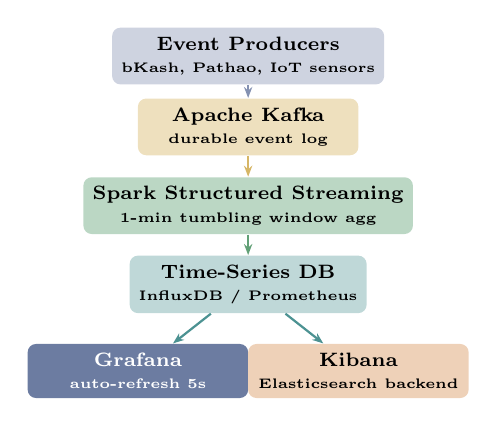
\begin{tikzpicture}[
          box/.style={rectangle, rounded corners=3pt, minimum width=2.8cm,
                      minimum height=0.65cm, font=\scriptsize\bfseries, align=center},
          arr/.style={-{Stealth[length=4pt]}, thick}
        ]
        \node[box, fill=PUNavy!20] (prod) at (0, 5.2)
              {Event Producers\\{\tiny bKash, Pathao, IoT sensors}};
        \node[box, fill=PUGold!30] (kaf)  at (0, 4.3)
              {Apache Kafka\\{\tiny durable event log}};
        \node[box, fill=PUGreen!30] (sp)  at (0, 3.3)
              {Spark Structured Streaming\\{\tiny 1-min tumbling window agg}};
        \node[box, fill=PUTeal!25] (tsdb) at (0, 2.3)
              {Time-Series DB\\{\tiny InfluxDB / Prometheus}};
        \node[box, fill=PUNavy!60, text=white] (graf) at (-1.4, 1.2)
              {Grafana\\{\tiny auto-refresh 5s}};
        \node[box, fill=PUOrange!30] (kib)  at (1.4, 1.2)
              {Kibana\\{\tiny Elasticsearch backend}};

        \draw[arr, PUNavy!50]  (prod)--(kaf);
        \draw[arr, PUGold!70]  (kaf)--(sp);
        \draw[arr, PUGreen!70] (sp)--(tsdb);
        \draw[arr, PUTeal!70]  (tsdb)--(graf);
        \draw[arr, PUTeal!70]  (tsdb)--(kib);
      \end{tikzpicture}
      \end{center}
      \vspace{4pt}
      \begin{alertblock}{WebSocket vs.\ Poll}
        \small Grafana polls the TSDB on a schedule (5s refresh).  For sub-second updates (stock tickers, live election counts), the server \textbf{pushes} updates via WebSocket --- the browser chart re-renders on each push event (D3.js + WebSocket).
      \end{alertblock}
  \end{columns}
\end{frame}

%================================================================
\section{Visualization Tools Landscape}
%================================================================

\begin{frame}{Tools Landscape: Choosing the Right Tool}
  \centering
  \renewcommand{\arraystretch}{1.5}
  \begin{tabular}{p{2.4cm}p{2.8cm}p{3.2cm}p{2.0cm}p{1.6cm}}
    \toprule
    \textbf{Tool} & \textbf{Best For} & \textbf{Data Source} & \textbf{Scale} & \textbf{Real-time} \\
    \midrule
    \textbf{Tableau} &
      Business dashboards, drag-and-drop BI &
      Spreadsheets, SQL, Spark, Hive &
      Millions of rows &
      Limited \\
    \textbf{Power BI} &
      Microsoft ecosystem, executive reports &
      Azure, Excel, SQL Server, REST API &
      Millions of rows &
      Limited \\
    \textbf{D3.js} &
      Custom interactive web visualizations &
      JSON, CSV, REST APIs &
      Flexible (client-side) &
      Yes (WebSocket) \\
    \textbf{Grafana} &
      Real-time metrics, ops dashboards &
      InfluxDB, Prometheus, Elasticsearch &
      Millions of data points &
      Yes (5s poll) \\
    \textbf{Apache Superset} &
      Open-source BI on data lakes &
      Presto, Hive, Spark SQL, PostgreSQL &
      Billions of rows &
      Limited \\
    \textbf{Kibana} &
      Log analytics, search exploration &
      Elasticsearch only &
      Billions of docs &
      Yes \\
    \bottomrule
  \end{tabular}
  \vspace{8pt}
  \begin{columns}[T]
    \column{0.48\textwidth}
      \begin{block}{Decision Heuristic}
        \small If your audience is \textbf{business users} $\to$ Tableau / Power BI.  If you need \textbf{custom interactive} charts on the web $\to$ D3.js.  If you need \textbf{real-time ops} monitoring $\to$ Grafana.  If you need \textbf{open-source BI on a Hadoop/Spark data lake} $\to$ Apache Superset.
      \end{block}
    \column{0.48\textwidth}
      \begin{alertblock}{D3.js: Why It Matters}
        \small D3 (\textbf{D}ata-\textbf{D}riven \textbf{D}ocuments) binds data to DOM elements.  Any SVG shape (circle, rectangle, path) can be driven by a data value.  This generality makes D3 the engine behind the \textit{New York Times} interactive graphics, The Guardian data journalism, and the NYT 2016/2020 election night needle.
      \end{alertblock}
  \end{columns}
\end{frame}

%================================================================
\section{Ivy League Alignment}
%================================================================

\begin{frame}{Data Visualization in Top University Curricula}
  \begin{columns}[T]
    \column{0.55\textwidth}
      \begin{block}{Harvard CS171 — Visualization (Pfister \& Borkin)}
        \small Harvard's dedicated visualization course, widely regarded as the gold standard:
        \begin{itemize}
          \item \textbf{Week 1} opens with Tufte's data-ink ratio and Anscombe's Quartet as the canonical argument for visualization
          \item \textbf{D3.js} is the mandatory implementation framework --- all assignments are interactive SVG charts in the browser
          \item \textbf{Shneiderman's mantra} is the grading rubric for interaction design: students lose marks if their dashboard does not implement overview $\to$ zoom $\to$ detail
          \item \textbf{Streaming data lab}: students wire a Kafka consumer to a D3.js chart via WebSocket and visualise Twitter sentiment in real time at 1{,}000 tweets/minute
          \item CS171 final projects have been published on the BBC, Boston Globe, and in academic visualization conferences
        \end{itemize}
      \end{block}

    \column{0.42\textwidth}
      \begin{exampleblock}{Stanford CS246 — MMDs (Leskovec)}
        \small Stanford uses visualization as an \textbf{analysis tool}, not just a presentation tool:
        \begin{itemize}
          \item t-SNE and UMAP projections of high-dimensional graph embeddings help students validate whether their community detection algorithms produce meaningful clusters
          \item Choropleth maps of PageRank scores over a geographic web graph reveal that high-authority pages cluster geographically --- an unexpected analytical insight discovered through visualization
        \end{itemize}
      \end{exampleblock}
      \vspace{4pt}
      \begin{alertblock}{MIT 6.859 — Interactive Data Visualization}
        \small MIT's visualization course focuses on \textbf{perceptual psychology}: why do humans judge bar length more accurately than angle (Pie chart problem)?  Why is color hue effective for categorical but not quantitative variables?  The Munsell color model, pre-attentive attributes, and Gestalt principles are covered alongside D3.js implementation.
      \end{alertblock}
  \end{columns}
\end{frame}

%================================================================
\section{Student Assessment Pool}
%================================================================

\begin{frame}{Assessment\textemdash MCQ Set A \hfill\small\textit{CLO3}}
  \begin{exampleblock}{Instructions}
    Select the single best answer.  Correct answers \textbf{bolded} for instructor reference.
  \end{exampleblock}
  \vspace{8pt}
  \begin{itemize}
    \item[\textbf{Q1.}] Edward Tufte's ``data-ink ratio'' principle states that a visualization should:
    \begin{enumerate}[(a)]
      \item Use more colours to highlight different categories of data
      \item \textbf{Maximise the fraction of ink devoted to representing actual data, removing all decorative elements}
      \item Use ink sparingly to reduce printing costs
      \item Always include data labels using a different ink colour from the chart body
    \end{enumerate}
  \end{itemize}
  \vspace{8pt}
  \begin{itemize}
    \item[\textbf{Q2.}] Which visualization type is most appropriate for showing the \textbf{distribution and spread} of a continuous variable?
    \begin{enumerate}[(a)]
      \item Pie chart \quad (b) Line chart \quad (c) \textbf{Histogram} \quad (d) Treemap
    \end{enumerate}
  \end{itemize}
  \vspace{8pt}
  \begin{alertblock}{Instructor Notes}
    \textbf{Q1:} Option (c) is a classic distractor --- the data-ink ratio is about what the ink \textit{encodes}, not how much is used.  A chart with one thick bar encoding one important value has a high data-ink ratio.  \textbf{Q2:} A pie chart (a) shows part-to-whole; a line chart (b) shows change over time; a treemap (d) shows hierarchical proportions.  Only the histogram (c) shows the shape of a continuous distribution.
  \end{alertblock}
\end{frame}

%----------------------------------------------------------------
\begin{frame}{Assessment\textemdash MCQ Set B \hfill\small\textit{CLO3}}
  \vspace{6pt}
  \begin{itemize}
    \item[\textbf{Q3.}] Shneiderman's visualization mantra begins with which step?
    \begin{enumerate}[(a)]
      \item Details first, then overview
      \item \textbf{Overview first, zoom and filter, then details on demand}
      \item Filter first, then provide an overview
      \item Details on demand first, then zoom out
    \end{enumerate}
  \end{itemize}
  \vspace{8pt}
  \begin{itemize}
    \item[\textbf{Q4.}] Which visualization tool is \textbf{best suited} for a real-time production operations dashboard monitoring server metrics and application error rates with 5-second refresh intervals?
    \begin{enumerate}[(a)]
      \item Tableau \quad (b) D3.js \quad (c) Power BI \quad (d) \textbf{Grafana}
    \end{enumerate}
  \end{itemize}
  \vspace{8pt}
  \begin{alertblock}{Instructor Notes}
    \textbf{Q3:} Options (a), (c), and (d) invert the mantra.  Students who select (c) ``filter first'' have confused the interaction sequence --- filtering is only meaningful after the user has seen the overview and identified what to filter.  \textbf{Q4:} Tableau (a) and Power BI (c) support limited scheduled refresh but are not designed for second-level streaming metrics.  D3.js (b) can do real-time with WebSockets but requires custom development; Grafana (d) natively integrates with time-series databases (InfluxDB, Prometheus) for live dashboards.
  \end{alertblock}
\end{frame}

%----------------------------------------------------------------
\begin{frame}{Assessment\textemdash True / False \hfill\small\textit{CLO3}}
  \begin{block}{Instructions}
    State True or False and provide a \textbf{one-sentence justification} for full marks.
  \end{block}
  \vspace{4pt}
  \centering
  \renewcommand{\arraystretch}{1.6}
  \begin{tabular}{p{9.0cm}c}
    \toprule
    \textbf{Statement} & \textbf{Answer} \\
    \midrule
    1.\ A pie chart is a recommended choice for comparing more than 5 categories. &
    \alert{\textbf{False}} \\
    2.\ Hexbin plots are an effective technique for reducing overplotting when visualising millions of data points. &
    \textbf{True} \\
    3.\ D3.js generates static PNG or PDF image files as its primary output format. &
    \alert{\textbf{False}} \\
    4.\ Choropleth maps are used to visualise the geographic distribution of a quantitative variable. &
    \textbf{True} \\
    \bottomrule
  \end{tabular}
  \vspace{6pt}
  \begin{exampleblock}{Model Justifications}
    \small \textbf{1:} With $>$5 categories, human perception of arc angles degrades; a horizontal bar chart ordered by value is always more readable.  \textbf{3:} D3.js binds data to \textbf{SVG DOM elements} in a web browser --- output is interactive, scalable vector graphics that update dynamically, not static image files.  \textbf{4:} A choropleth uses colour intensity to encode a quantitative variable (e.g., dengue incidence rate per 100{,}000 population) mapped onto geographic polygons (districts, divisions, countries).
  \end{exampleblock}
\end{frame}

%----------------------------------------------------------------
\begin{frame}{Assessment\textemdash Descriptive Questions \hfill\small\textit{CLO3}}
  \begin{block}{Instructions}
    Answer each question in \textbf{100--150 words}.  Include diagrams where indicated.
  \end{block}
  \vspace{8pt}
  \begin{itemize}
    \item[\textbf{D1.}] Explain Tufte's \textbf{data-ink ratio} principle.  Provide a ``before and after'' example: describe a cluttered bar chart (what chart-junk elements are present) and then describe the clean version after applying the principle.
  \end{itemize}
  \vspace{8pt}
  \begin{itemize}
    \item[\textbf{D2.}] What is \textbf{overplotting}?  Describe \textbf{three techniques} to address it when visualising millions of data points in a scatterplot.  For each technique, explain what information it preserves that the original overplotted chart lost.
  \end{itemize}
  \vspace{8pt}
  \begin{itemize}
    \item[\textbf{D3.}] What is a \textbf{data cube}?  How does pre-aggregating a billion-row fact table into a data cube enable interactive visualization at sub-second latency?  What is the trade-off of this approach?
  \end{itemize}
\end{frame}

%----------------------------------------------------------------
\begin{frame}{Assessment\textemdash Analytical Questions \hfill\small\textit{CLO3}}
  \begin{block}{Instructions}
    Answer in \textbf{200--300 words} with step-by-step reasoning.  Reference Shneiderman's taxonomy and Tufte's principles where applicable.
  \end{block}
  \vspace{6pt}
  \begin{itemize}
    \item[\textbf{A1.}] \textbf{Public Health Dashboard Design:}\\
    A DGHS public health dashboard needs to communicate:
    \begin{itemize}
      \item (a) COVID-19 confirmed case counts by district over 24 months
      \item (b) Real-time hospitalisation rate updated every 5 minutes
      \item (c) Demographic breakdown (age group, gender) of confirmed cases
    \end{itemize}
    For each sub-requirement: specify the appropriate visualization type, justify using Shneiderman's data-type taxonomy, identify which big data visualization challenge applies (if any), and name the tool you would use.  Apply Tufte's data-ink principle to state one specific chart-junk element to eliminate.
  \end{itemize}
  \vspace{6pt}
  \begin{itemize}
    \item[\textbf{A2.}] \textbf{Streaming Sentiment Visualization:}\\
    Design a complete visualization system for a streaming Twitter (X) sentiment analysis pipeline processing \textbf{10{,}000 tweets per second}.  Specify: (a) which Kafka aggregation window you would use and why; (b) which chart types best convey sentiment drift over time and topic clustering; (c) how you would handle the velocity challenge at the visualization layer without overloading the browser; (d) which tools form the pipeline from Kafka to browser render.
  \end{itemize}
\end{frame}

%================================================================
\section*{Textbook References}
%================================================================

\begin{frame}{Textbook \& Reading References}
  \begin{block}{Primary Textbooks for Week 9}
    \begin{itemize}
      \item \textbf{[SA]}\ Acharya \& Chellappan. \textit{Big Data and Analytics}, Wiley, 2015.
            \hfill\textbf{Ch.\ 10}
            \begin{itemize}
              \small\item Ch.\,10: Data Visualization --- chart types, big data visualization tools, dashboard design
            \end{itemize}
      \item \textbf{[TE]}\ Erl, Khattak \& Buhler. \textit{Big Data Fundamentals}, Prentice Hall, 2016.
            \hfill\textbf{Ch.\ 12}
            \begin{itemize}
              \small\item Ch.\,12: Big Data Analysis and Visualization --- analytical techniques, output communication
            \end{itemize}
    \end{itemize}
  \end{block}
  \vspace{4pt}
  \begin{exampleblock}{Seminal Works (covered in Week 9, Part 2)}
    \begin{itemize}
      \small
      \item Tufte, E.\ R.\ (1983). \textbf{\textit{The Visual Display of Quantitative Information.}} Graphics Press. [Required at Harvard, Yale, Stanford --- the founding text of analytical visualization]
      \item Shneiderman, B.\ (1996). \textbf{The Eyes Have It: A Task by Data Type Taxonomy for Information Visualizations.} \textit{IEEE Symposium on Visual Languages.} [Defines the overview-zoom-filter-details mantra and seven data types]
      \item Bostock, M., Ogievetsky, V., \& Heer, J.\ (2011). \textbf{D$^3$: Data-Driven Documents.} \textit{IEEE Transactions on Visualization and Computer Graphics.} [Introduces D3.js; most cited visualization systems paper of the 2010s]
    \end{itemize}
  \end{exampleblock}
\end{frame}

%----------------------------------------------------------------
\begin{frame}[c]
  \begin{center}
    {\Large\bfseries Questions \& Discussion}\\[10pt]
    {\large Week 9, Part 1 $\;\mid\;$ CSE 4345 Big Data Analytics}\\[8pt]
    \textcolor{PUGray}{\rule{7cm}{0.5pt}}\\[10pt]
    \begin{quote}
      \itshape ``Above all else, show the data.''
    \end{quote}
    \hfill\textemdash\ Edward R.\ Tufte, \textit{The Visual Display of Quantitative Information}, 1983
    \vspace{12pt}
    \begin{block}{\centering Next Lecture: Week 9, Part 2}
      \centering
      Seminal Papers: Tufte (1983) $\cdot$ Shneiderman (1996) $\cdot$ Bostock et al.\ D$^3$ (2011)\\[4pt]
      \small Case Study: \textbf{New York Times Graphics Desk} ---
      D3.js real-time election visualizations, communicating uncertainty with probability distributions, live data streaming as results arrive on election night
    \end{block}
    \vspace{6pt}
    \textbf{Reading before Part 2:}\ \textbf{[SA]} Ch.\,10 $\cdot$ Tufte (1983) Ch.\,1--2 (data-ink ratio, chart junk)
  \end{center}
\end{frame}

%=================================================================
\end{document}
%=================================================================
